\documentclass[serif,xcolor=pdftex,dvipsnames,table,hyperref={bookmarks=false,breaklinks}]{beamer}

%%%%%%%%%%%%%%%%
% Change the macros below to configure the title slides
% for your course.
\newcommand{\coursename}{COMPSCI 590N}
\newcommand{\instructor}{Roy J. Adams}
\newcommand{\university}{University of Massachusetts Amherst}
\newcommand{\department}{College of Information and Computer Sciences}
%%%%%%%%%%%%%%%%

\newcommand\HUGE{\@setfontsize\Huge{50}{60}}

\newcommand{\settitlecard}[2]{
  \title[\coursename  Lecture #1] 
    {\coursename \\ Lecture #1: #2}
     \author[\instructor]{\instructor}
     \institute[\university]{
     \department\\
     \university
   }
\date{}
}

\newcommand{\maketitlepage}{
  \begin{frame}
  \titlepage
  %\center{
    %If you use the slides unmodified, retain the attribution below
  %  \tiny{Slides by Roy J. Adams (rjadams@cs.umass.edu). 
    %If you modify the slides, please retain the alternate attribution below
    %\tiny{Based on slides by Roy J. Adams (rjadams@cs.umass.edu). \\    
  %  }                                              
  %}  
  \end{frame}
}

\AtBeginSection[]
{
  \begin{frame}<beamer>{Outline}
    \tableofcontents[currentsection,subsectionstyle=hide]
  \end{frame}
}


\newcommand{\cut}[1]{}

\newcommand{\iconbox}[4]{
  \only<#1-#2>{
    \begin{columns}[T]
      \column{0.5in}
           \includegraphics[width=0.5in]{#3}
       \column{3.7in}
            #4
    \end{columns}
    \medskip
    \medskip
    \medskip
  }
}

\mode<presentation>{
  \usepackage{../beamertheme589theme}
  \setbeamercovered{invisible}
}

\mode<handout>{
  \usepackage{../beamertheme589theme}
  \setbeamercovered{transparent}
}


\usepackage[english]{babel}
\usepackage[latin1]{inputenc}
\usepackage{times}
\usepackage[T1]{fontenc}
\usepackage{amsmath}
\usepackage{amssymb}
\usepackage[noend]{algorithmic}
\usepackage{algorithm}
\usepackage{listings}
\usepackage{tcolorbox}
\usepackage{xmpmulti}

\renewcommand\mathfamilydefault{\rmdefault}

\newcommand{\setA}{\mathcal{A}}
\newcommand{\setB}{\mathcal{B}}
\newcommand{\setS}{\mathcal{S}}
\newcommand{\setV}{\mathcal{V}}
\DeclareMathOperator*{\union}{\bigcup}
\DeclareMathOperator*{\intersection}{\bigcap}
\DeclareMathOperator*{\Val}{Val}
\newcommand{\mbf}[1]{{\mathbf{#1}}}
\DeclareMathOperator*{\argmax}{arg\,max}
\DeclareMathOperator*{\argmin}{arg\,min}
\DeclareMathOperator*{\sign}{sign}
\newcommand{\deriv}[2]{\frac{\partial{#1}}{\partial{#2}}}

\lstdefinestyle{custompython}{
  belowcaptionskip=1\baselineskip,
  breaklines=true,
  frame=single,
  xleftmargin=\parindent,
  language=Python,
  showstringspaces=false,
  basicstyle=\footnotesize\ttfamily,
  keywordstyle=\bfseries\color{green!40!black},
  commentstyle=\itshape\color{purple!40!black},
  identifierstyle=\color{blue},
  stringstyle=\color{orange},
}
\lstset{style=custompython}

\makeatletter
\renewcommand*\env@matrix[1][*\c@MaxMatrixCols c]{%
  \hskip -\arraycolsep
  \let\@ifnextchar\new@ifnextchar
  \array{#1}}
\makeatother

\newcommand\norm[1]{\left\lVert#1\right\rVert}


\settitlecard{3}{Classes and Representing Numbers}

\begin{document}

\maketitlepage

% \section{Preliminaries}
% \subsection{Foo}
%
%
% \begin{frame}[t]{Reminders}
% 	\begin{itemize}[<+->]
% 		\item Assignment 1 due Tonight (09/13) by 11:59pm
% 		\begin{itemize}[<+->]
% 			\item Check Piazza
% 			\item Check your return types
% 		\end{itemize}
% 		\item Quiz 2 is going out tonight after class. Fewer questions, but they are a little longer.
% 		\item If you cannot make my office hours, feel free to email me and set up another time.
% 	\end{itemize}
% \end{frame}

\section{Modules and Objects}
\subsection{Foo}

% \begin{frame}[t]{Scoping}
%
% \end{frame}

\begin{frame}[t,fragile]{Importing Functions}
	\begin{itemize}[<+->]
		\item \textbf{Modules} are Python packages, usually a collection of functions and variable, that can be used in other programs.
		\item Load modules into your code using an \textbf{import} statement.
	\end{itemize}
	\pause
	\begin{tcolorbox}
		\begin{verbatim}
			import <module_name> # imports a module
		\end{verbatim}
	\end{tcolorbox}
	%
	% \pause
	% \centering
	% \Huge{DEMO}
\end{frame}

\begin{frame}[t]{Useful Built-in Modules}
	Python has a number of very useful built-in modules:

	\begin{itemize}[<+->]
		\item \textbf{string:} operations on strings.
		\item \textbf{math:} standard math functions such as: log, exp, sine, etc.
		\item \textbf{itertools:} functions for manipulating sequences such as: combinations, permutations, cross product, etc.
	\end{itemize}
	% string
	% math
	% itertools
	\pause
	\centering
	\Huge{DEMO}
\end{frame}

\begin{frame}[t]{Object Oriented Programming}
	\Huge{DEMO}
\end{frame}

\begin{frame}[t,fragile]{Classes}
	Create new object types in Python by defining a \textbf{class}.
	\pause
	\begin{tcolorbox}
		\begin{verbatim}
			class <class_name>:
			   def __init__(self,<args>):
			      self.<member_variable> = <expression>
			      <body>
					
			   def <member_function>(self,<args>):
			      <body>
		\end{verbatim}
	\end{tcolorbox}
\end{frame}

\begin{frame}[t,fragile]{What are objects?}
	\begin{itemize}[<+->]
		\item Objects, like functions, are a tool for organizing programs.
		\item An object consists of:
		\begin{enumerate}[<+->]
			\item A collection of related information.
			\item A set of operations to manipulate and access that information.
		\end{enumerate}
		\item The information is stored as \textit{instance variables}.
		\item The operations are called \textit{methods}.
		\item Collectively the methods and instance variables are called \textit{attributes}.
	\end{itemize}
	
	\pause
	\begin{block}{Dog Example:}
		\begin{itemize}[<+->]
			\item \textbf{Instance variables}:
			\begin{itemize}[<+->]
				\item \verb|name| and \verb|tricks|
			\end{itemize}
			\item \textbf{Methods:}
			\begin{itemize}[<+->]
				\item \verb|bark|, \verb|teach_trick|, and \verb|do_trick|
			\end{itemize}
		\end{itemize}
	\end{block}
	
\end{frame}

% \section{Miscelaneous Python}
% \subsection{Foo}
%
% \begin{frame}[t,fragile]{List Comprehensions}
% 	Python supports a concept called \textbf{list comprehensions} which can be used to conveniently create sequences.
% 	\pause
% 	\begin{block}{Class Definitions}
% 		\begin{verbatim}
% 			[<expresion> for <var> in <sequence>]
% 		\end{verbatim}
% 	\end{block}
% 	\pause
% 	\centering
% 	\Huge{DEMO}
%
% \end{frame}

% \begin{frame}[t]{Functional programmingesque Python}
% 	Python includes a number of functions
% \end{frame}
%
% \begin{frame}[t]{Misc}
% 	% with
% 	% None
% \end{frame}

\section{Intro to Numerical Computing}
\subsection{Foo}

\begin{frame}[t]{Numerical Computing}
	\centering
	\Large{\textbf{Numerical computing} is the approximation of continuous values and functions on a computer with finite precision.}
	
	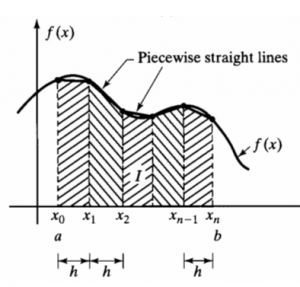
\includegraphics[width=2in]{../Figures/numerical_integration.png}
\end{frame}

\begin{frame}[t]{Representing Numbers}
	Before we can approximate functions, we need to represent numbers:
	\pause
	\begin{itemize}[<+->]
		\item The set of integers is countably infinite.
		\item The set of real numbers is continuous and uncountably infinite.
		\item But the set of numbers representable by a computer is finite...
	\end{itemize}
\end{frame}

\begin{frame}[t]{Integer Representation}
	Given a fixed number of bits (usually 32 or 64), we can create the following mapping:
	
	\pause
	\centering
	\begin{tabular}{|r|r|}\hline
		integral number & bit representation\\\hline\hline
		0 & 00000000\\
		1 & 00000001\\
		2 & 00000010\\
		3 & 00000011\\
		4 & 00000100\\
		\vdots & \vdots\\
		254 & 11111110\\
		255 & 11111111\\\hline
	\end{tabular}
	
	\pause
	\begin{itemize}[<+->]
		\item Shift the mapping to store negative numbers: $0000000_2 = -125$ and $11111111_2 = 126$. 
	\end{itemize}
		
		% meaning we can represent number up to ~$2.1\cdot 10^9$ and ~$9.2\cdot 10^18$ respectively.
\end{frame}

\begin{frame}[t]{Integer Representation}
	\centering
	\begin{block}{Binary Integers}
		Given $n$ bits, $b_1,...,b_n\in \{0,1\}$, we map binary values to integer values as follows: 
		\Large{$$(b_nb_{n-1}...b_2b_1b_0)_2 = \sum_{i=0}^n b_i2^i = x$$}
	\end{block}
	
	\pause
	For example:
	\Large{$$0101_2 = 0\cdot2^3 + 1\cdot2^2 + 0\cdot2^1 + 1\cdot2^0 = 5$$}
\end{frame}

\begin{frame}[t]{Real Representations}
	\begin{block}{Fixed Point}
		Represent real numbers as integers that are scaled by a fixed scaling factor, $d$. For example: Let $d = 1000$, then
		
		$$1.23 = \frac{12300}{d}$$
	\end{block}
	\pause
	\begin{itemize}[<+->]
		\item This is equivalent to shifting the decimal.
		\item $d$ is usually a multiple of $2$.
		\item Restricted by the range of representable integers.
		\item \textbf{Observation:} Between 0 and 1, we would usually like a finer discretization, but between 1000 and 1001, we may be ok with a rough discretization.
	\end{itemize} 
\end{frame}

\begin{frame}[t]{Real Representations}
	\begin{block}{Floating Point}
		Rewrite a number, $x$, in scientific notation $x = a\cdot 10^b$. Then, $x$ can be stored by storing $a$ as a fixed point and $b$ as an integer. Floating point numbers use a fixed number of digits for $a$, known as the \textit{mantissa}, and $b$, known as the \textit{exponent}:
		
		\pause
		\centering
		\begin{tabular}{|r|r|r|}\hline
			$x$ & $a$ & $b$\\\hline
			123.456 & 1.23456 & 2\\
			100000 & 1.00000 & 5\\
			0.00025 & 2.50000 & -4\\\hline
		\end{tabular}
	\end{block}
	\pause
	\begin{itemize}[<+->]
		\item Floating point numbers naturally have finer granularity nearer zero.
	\end{itemize}
\end{frame}

\begin{frame}[t]{Floating Point Limitations}
	\begin{itemize}[<+->]
		\item Typically, 54 bits are used for the mantissa and 10 bits are used for the exponent.
		\item This results in:
		\begin{itemize}[<+->]
			\item The largest possible float is $\approx 10^{308}$.
			\item The smallest possible float is $\approx 10^{-308}$.
			\item The distance between 1.0 and the next largest number is $\approx 10^{-16}$.
		\end{itemize}
		\item Because we can only represent finite numbers, we must rely on rounding and approximation which can lead to errors if you are not careful.
	\end{itemize}
\end{frame}

% \begin{frame}[t]{Rounding in Action}
% 	Can a $10^-16$ make a difference?
% 	\begin{itemize}[<+->]
% 		\item Ca
% 		\item This results in:
% 		\begin{itemize}[<+->]
% 			\item The largest possible float is $\approx 10^{308}$.
% 			\item The smallest possible float is $\approx 10^{-308}$.
% 			\item The distance between 1.0 and the next largest number is $\approx 10^-16$.
% 		\end{itemize}
% 		\item Because we can only represent finite numbers, we must rely on rounding and approximation.
% 	\end{itemize}
% \end{frame}

\begin{frame}[t]{Overflow/Underflow}
	\pause
	\begin{block}{Overflow}
		Overflow occurs when an expression results in a number that is too \textbf{large} to be represented.
	\end{block}
	
	\pause
	\begin{block}{Underflow}
		Underflow occurs when an expression results in a number that is too \textbf{small} to be represented.
	\end{block}
	
	\pause
	\centering
	\Huge{Demo}
	
\end{frame}

\begin{frame}[t]{Representability}
	\begin{itemize}[<+->]
		\item Not all decimal numbers are representable using a binary, floating point representation.
		\item Example: 0.1
		\item The set of representable numbers is not closed under standard arithmetic. That is, adding, subtracting, multiplying, or dividing representable numbers may result in an unrepresentable number.
		\item Example: 1.0/10.0 = 0.1
	\end{itemize}
	
	\pause
	\centering
	\Huge{Demo}
\end{frame}

\begin{frame}[t]{Working with floating point numbers}
	\begin{itemize}[<+->]
		\item Scale your variables or work in log space to avoid overflow and underflow.
		\item Avoid using == to compare floating point numbers. Instead compare with a tolerance: $|x - y| < \epsilon$
	\end{itemize}
	
	\pause
	\centering
	\Huge{Demo}
\end{frame}

\begin{frame}[t]{Rounding in Action}
	Can a $10^{-16}$ make a difference?
	\pause
	\begin{block}{Patriot Missile Failure}
		\begin{itemize}[<+->]
			\item Missile defense system failed to target an incoming missile due to a rounding error.
			\item The error was caused by counting time in tenths of seconds (+= 0.1).
			\item As in our demo, this resulted in accumulating errors because 0.1 is not representable.
			\item Incorrect timestamps were then used to incorrectly calculate distance and speed of an incoming missile.
		\end{itemize}
	\end{block}
\end{frame}

\end{document}
